\section{Mindfulness}
Mindfulness has its roots in Buddhism and yogic tradition and is described as a non-elaborative and non-judgmental awareness of the present moment \cite{Kabat1982,Zeidan2012,Zeidan2016,Tang2017}. Within a mindfulness stage one is focusing from one moment to the other and is aware of emotional, cognitive and sensory events. Those events are perceived as temporary, fading and changeable. Moreover one is neither rating nor reacting cognitive or emotional to those events. The mental state of mindfulness can be achieved by mental training. \cite{Zeidan2012,Zeidan2016}  Thus can be said that mindfulness meditation is training of the mind \cite{Tang2017}. 

Since thoughts and emotions are involved in the perception of pain, mindfulness provides the ability to relieve pain. Mindfulness cannot cure pain, but the patients will be able to deal with the pain easier and reduce the fear associated with pain. Thereby the patients engage more in their treatment instead of relying and focusing on the effects of medication. \cite{Jacob2016}
Often used methods to reach mindfulness are meditation and yoga practice \cite{Kabat1982}.  In this study meditation was used, because physical limitations are not affecting the meditation practice and no prior knowledge is needed \cite{Tang2017}.


\subsection{Meditation classification}
The most well practiced types of meditation are focused attention (FA) and open monitoring (OM). \cite{Zeidan2016} FA is the training of concentration. The subjects keep their focus at an object or specific thing. Hereby the flow of breath is often used.  If any disturbance comes by, like a thought, sound or other environmental distractions, which will often lead to a drift in attention, the person should always bring the attention back to the focus. \cite{Zeidan2016} OM is the cultivation of open presence. The mind is open to anything, not focusing on any specific thing, just being in the present. If any thought or disturbance comes by, the thought or sensation should be noticed briefly, but then left without thinking more over it. FA is used to slide into OM, therefore it is necessary to master FA before one can reach OM. \cite{Perlman2016, Zeidan2016,Kabat1982} Hence the chosen meditation practice in this study is FA.


%This kind of meditation has been shown to reduce pain more compared to FA, likely because the areas of the brain affected during this form of meditation is \cite{Perlman2010}

%FA and OM can alter pain in different ways...
%OM is more effective in reducing pain after extensive meditation training compared to FA. \cite{Varilly2012}

%(.....MAYBE WE NEED SOME KIND OF REASONING TO WHY WE CHOOSE TO LOOK INTO MINDFULNESS MEDITATION, LIKE A SUMMARY OF ALL THE METHODS BEFORE GOING INTO MINDFULNESS MEDITATION, AND THEN DIG DEEPER INTO THE FACTS OF MINDFULNESS MEDITATION....)

\subsection{Mechanisms of mindfulness}

Previous research indicates that mindfulness meditation is promising for relieving pain, even though the research is limited, and the mechanisms behind mindfulness meditation are not fully understood yet \cite{Perlman2010}. 
Studies show that enhanced emotion regulation, cognitive control, acceptance and positive mood have been linked with health benefits as well as pain modulation. These mechanisms are modulated during mindfulness meditation practice.

With mindfulness meditation one is able to take the attention away from the emotional component of pain. Therefore meditation practice can reduce the brain process areas related to anticipation of pain, which does not imply that meditation reduce the brain process related with pain. \cite{Brown2010}
Pain as well as meditation alter sensory, cognitive and affective dimensions of subjective experience. Therefore brain areas activated during meditation and nociception should be interconnected in a way. \cite{Zeidan2011}

A study by Perlman et al. \cite{Perlman2010} shows that practicing meditation could not lower the intensity of pain, but instead lower pain unpleasantness in the participants. \cite{Zeidan2012, Perlman2010} Similarly, a study by Brown and Jones et al. \cite{Brown2010} showed that the greater the experience is with meditation the lower the perception of pain unpleasantness. This results in lower activation of the right Inferior Parietal Cortex (IPC) and Midcingulate Cortex (MCC).  This findings are supported by a study by Lutz et al. \cite{Lutz2013} which shows that unpleasantness rating of pain decrease with meditation experience.
 

%The typical response, when using a placebo analgesia is increased activation of the dorselateral prefrontal cortex during pain anticipation. This effect predicts reductions in pain perception and activity of pain related brain regions. Mindfulness meditation does not involve dorselateral prefrontal cortex activation. \cite{Zeidan2012}


%The findings on mindfulness meditation and pain modulation are split, but experiments in controlled settings are still needed to confirm, if the effect of mindfulness meditation works on pain modulation. \cite{Zeidan2012, Perlman2010}

%****COMENTS FROM BO*****
A study by Gard et al. \cite{Gard2012} reported that the brain pattern related with pain modulation during mindfulness differs to other pain coping strategies. An increased activation in the rostral Anterior Cingulate Cortex (ACC) and the ventromedial Prefrontal Cortex (PFC) in the anticipation of pain stage was found for mindfulness practitioners. The activation of this areas has been identify with positive emotions. Furthermore, the study by Gard et al. \cite{Gard2012} found for mindfulness practitioners an increased activation in the rostral
ACC and ventromedial PFC while anticipating pain. As well as decreased activation in the bilateral lateral PFC and increased activation in the posterior insula and secondary somatosensory cortex (S2) when receiving a stimuli. Moreover, a study by Grant et al. \cite{Grant2012} showed that mindfulness practitioners have different neuronal responses to painful stimuli with a greater activation in the insula and thalamus and a decrease activity in PFC.

%\fxnote{....and then we need something like: or maybe a summary of all the methods and then saying, because of this and this, mindfulness meditation will be looked further upon as method for reliving pain...}

%The method of mindfulness meditation will be used for method to relief pain in this project.

%\section{Mindfulness meditation}
%Definition
Different brain regions are involved in the practice of mindfulness meditation. 

\begin{figure}[H]
	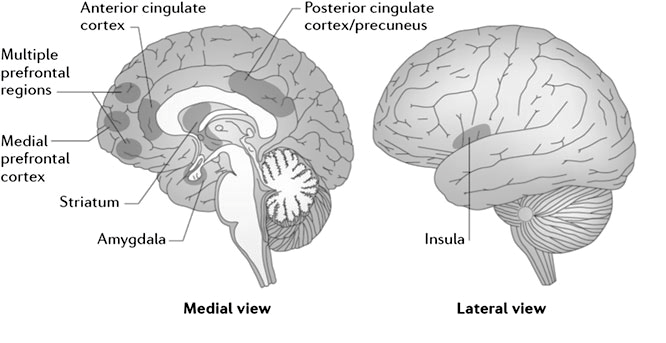
\includegraphics[width=0.9\textwidth]{figures/brain_meditation.png} 
	\caption{Specific regions in the brain involve when practicing mindfulness meditation \cite{Tang2017}.}
	\label{fig:brain_meditation}  
\end{figure}

Hence, the most involved in pain modulation via mindfulness meditation is the PFC and the ACC as illustrated in \figref{fig:brain_meditation}. Furthermore, striatum, insula and Default Mode Network (DMN), which includes the medial PFC and the Posterior Cingulate Cortex (PCC) are shown in \figref{fig:brain_meditation}. These regions play a big role in the effect of mindfulness meditation and are highly regulating the mechanisms of meditation which can generally be categorized into three categories: attention control, emotion regulation and self-awareness. 

%Figure \ref{fig:brain_meditation} shows an image of the brain and the regions involved in attention, emotion and self awareness. 
  
\begin{itemize}
	\item \textbf{Attention control} is the ability to maintain focus, for instance on the breath during FA meditation. This mechanism includes mainly ACC, PFC and the striatum, which are illustrated in \figref{fig:brain_meditation} as the red dots. Increased activity in the dorsal lateral PFC is required to hold an increased attention, as well as deactivation of the areas of the brain that makes the mind drift, which include the medial PFC. \cite{Tang2017}
	\item \textbf{Emotion regulation}
	includes the emotions that arise, when they occur and how they are experienced and expressed. This mechanism involves multiple prefrontal regions, limbic regions and striatum, which are regions primary regulating the emotional thoughts through the limbic system also responsible for goal setting. These regions are illustrated as green dots on \figref{fig:brain_meditation}. This need for regulating the emotional control is important because the participant needs to be able to handle boredom or negative mood during the meditation. Stronger subgenual and adjacent ventral ACC activity is present with meditation. This brain area is involved with emotion regulation and attention control. The dorsal lateral PFC and amygdala plays some role in regulation of emotion.  \cite{Tang2017}

	\item \textbf{Self-awareness} includes the awareness of oneself, the awareness of being conscious as well as meta-awareness, which is the awareness of the internal bodily state. Regions of the brain involves midline cortical structure DMN, ACC, the insula, medial PFC and PCC, as illustrated in \figref{fig:brain_meditation} as blue dots. Reduced activity in midline cortical structure including the DMN, more reduction in the posterior part PCC, than the anterior part medial PFC, but increased in perigenual ACC activity.  \cite{Tang2017}
\end{itemize}


\subsection{Stages of meditation}
Different expertise of meditation appear to modulate the dynamic balance between anterior and posterior midline networks involved in different aspects of self, cognitive self, bodily self and phenomenal experiential self. This reflects self-plasticity following meditation. 
The effort to get into the meditative state varies according to your experience level with meditation. Often this experience level can be divided into three stages, early, middle and advanced practice of meditation. These stages, illustrated in figure \ref{fig:meditation_stages}, determine the amount of effort to get into the meditative state. \cite{Tang2017} 

\begin{figure}[H]
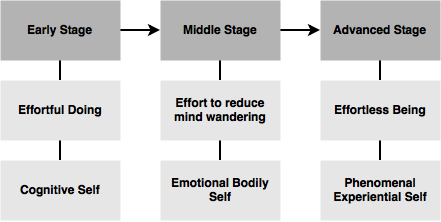
\includegraphics[width=0.8\textwidth]{figures/stages_of_meditation.png} 
	\caption{The three stages of meditation practice describe the effort, which is necessary, to get into the meditative state. \cite{Tang2017}}
	\label{fig:meditation_stages}  
\end{figure}  

In the early stage more mental effort is required. Here the dorsal lateral PFC and partial cortex are often involved and activated more. A stronger deactivation in the DMN occurs when more effort is used. With less effort, the ACC and striatum will participate more. \cite{Tang2017}

The neural mechanisms behind mindfulness meditation in relieving pain has been researched. Experiments with stimulation of nociceptive pain have shown an increase in active areas of the PFC while meditating. Participants express that they feel the pain but are able to deal with it better during meditation focusing on the breath. 
The mechanisms working in analgesia are not the same as the mechanisms during meditation, why the two methods do not interfere with each other. \cite{Jacob2016}

The different areas of the brain show either a reduction or increase in activity when performing meditation. Through meditation the person trains the mind, and specific regions will grow. \cite{Zeidan2012}


%*** Used for state of the art ***
%Examining long term meditators, the findings are a thicker gray matter in mid cingulate cortex and bilateral secondary somatosensory cortex, which are involved in pain related regions overlapping the functional effect. A correlation with the number of years practicing meditaiton and the mid cingulate was also found. This gives evidence to long lasting effects of meditation. \cite{Zeidan2012}
%
%However, short-term mindfulness training can have positive effect in pain relieve. The study by \cite{Zeidan2012} showed an effect of mindfulness meditation practice during four days for 20 min per session, even though most studies conduct the experiments for a period of more than six weeks. \cite{Zeidan2012}
